\phantomsection
\section*{\fontsize{12}{18}\selectfont Modulación y Demodulación.}
\addcontentsline{toc}{section}{Modulación y Demodulación}

\begin{justify}
    Son procesos fundamentales en los sistemas de comunicación electrónica, esenciales para transmitir información de manera eficiente y confiable.
\end{justify}

\phantomsection
\subsection*{\fontsize{12}{18}\selectfont Modulación.}
\addcontentsline{toc}{subsection}{Modulación}

\begin{justify}
    Es el proceso mediante el cual una señal de información se combina con una señal portadora de mayor frecuencia para facilitar su transmisión. Esta
    técnica permite que la información sea transportada de manera más efectiva a través de diversos medios. Las principales técnicas de modulación son:

    \begin{itemize}
        \item \textbf{\acrlong{am}:} La amplitud de la portadora varía en proporción a la señal de información.
        
        \item \textbf{\acrlong{fm}:} La frecuencia de la portadora se ajusta según las variaciones de la señal de información.
        
        \item \textbf{\acrlong{pm}:} La fase de la portadora cambia en función de la señal de información.
    \end{itemize}

    En sistemas digitales, se utilizan técnicas de modulación más avanzadas, como:

    \begin{itemize}
        \item \textbf{\acrlong{ask}:} La amplitud de la portadora cambia entre valores discretos para representar datos binarios.
        
        \item \textbf{\acrlong{fsk}:} La frecuencia de la portadora alterna entre valores predefinidos para representar bits.
        
        \item \textbf{\acrlong{psk}:} La fase de la portadora se desplaza en ángulos específicos para codificar información digital.
        
        \item \textbf{\acrlong{qam}:} Combina variaciones en amplitud y fase para transmitir más bits por símbolo, aumentando la eficiencia espectral.
    \end{itemize}

    \begin{equation}
        v(t) = V \sin(2\pi f t + \theta)
    \end{equation}

    donde
    \begin{equation*}
        \begin{array}{rl}
            v(t) & = \text{voltaje variable senoidalmente en el timepo}\\
            V & = \text{amplitud máxima (volts)}\\
            f & = \text{frecuencia (hertz)}\\
            \theta & = \text{desplazemiento de fase (radianes)}
        \end{array}
    \end{equation*}

    Resumen de las técnicas de modulación
\end{justify}

\begin{center}
    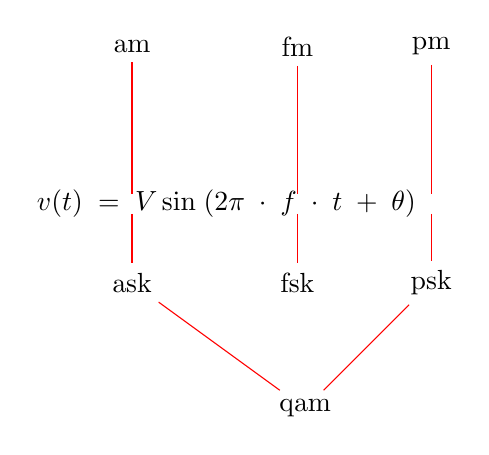
\begin{tikzpicture}
        % Encabezados
        % \node at (-3.5,3) {señal};
        % \node at (-3.5,2.6) {modulante};
        % \node at (3.5,3) {modulación};
        % \node at (3.5,2.6) {efectuada};

        % Modulación analógica
        \node (AM) at (-1.2, 3) {\acrshort{am}};
        \node (FM) at (0.9, 3) {\acrshort{fm}};
        \node (PM) at (2.6, 3) {\acrshort{pm}};

        % Ecuación con nodos de anclaje
        \node (eq) at (0,1) {\( v(t)\; =\; V\sin\; (2\pi\; \cdot\; f\; \cdot\; t\; +\; \theta) \)};

        % Agregar nodos invisibles en V, f y theta para conectar líneas
        \node (V) at (-1.2, 1) {};
        \node (f) at (0.9, 1) {};
        \node (theta) at (2.6, 1) {};

        % Conexión de modulaciones analógicas con sus respectivas partes en la ecuación
        \draw[red] (AM) -- (V);
        \draw[red] (FM) -- (f);
        \draw[red] (PM) -- (theta);

        % Modulación digital
        \node (ASK) at (-1.2, 0) {\acrshort{ask}};
        \node (FSK) at (0.9, 0) {\acrshort{fsk}};
        \node (PSK) at (2.6, 0) {\acrshort{psk}};

        % Conexión de modulación digital con la ecuación
        \draw[red] (V) -- (ASK);
        \draw[red] (f) -- (FSK);
        \draw[red] (theta) -- (PSK);

        % Modulación QAM
        \node (QAM) at (1, -1.6) {\acrshort{qam}};

        % Conexiones de QAM (ASK y PSK)
        \draw[red] (ASK) -- (QAM);
        \draw[red] (PSK) -- (QAM);
    \end{tikzpicture}
\end{center}

\phantomsection
\subsection*{\fontsize{12}{18}\selectfont Demodulación.}
\addcontentsline{toc}{subsection}{Demodulación}

\begin{justify}
    Es el proceso inverso a la modulación. Consiste en extraer la información original de la señal modulada recibida, recuperando así la señal de
    información para su procesamiento o interpretación.
\end{justify}

\phantomsection
\subsection*{\fontsize{12}{18}\selectfont Binary Phase Shift Keying (BPSK).}
\addcontentsline{toc}{subsection}{Binary Phase Shift Keying (BPSK)}

\begin{justify}
\end{justify}

\phantomsection
\subsection*{\fontsize{12}{18}\selectfont Quadrature Phase Shift Keying (QPSK).}
\addcontentsline{toc}{subsection}{Quadrature Phase Shift Keying (QPSK)}

\begin{justify}
\end{justify}

\phantomsection
\subsection*{\fontsize{12}{18}\selectfont Minimum Shift Keying (MSK).}
\addcontentsline{toc}{subsection}{Minimum Shift Keying (MSK)}

\begin{justify}
\end{justify}

\phantomsection
\subsection*{\fontsize{12}{18}\selectfont Binary Offset Carrier (BOC).}
\addcontentsline{toc}{subsection}{Binary Offset Carrier (BOC)}

\begin{justify}
\end{justify}

\phantomsection
\subsection*{\fontsize{12}{18}\selectfont Composite Binary Offset Carrier (CBOC).}
\addcontentsline{toc}{subsection}{Composite Binary Offset Carrier (CBOC)}

\begin{justify}
\end{justify}